\documentclass{article}
\usepackage{graphicx}
\usepackage{tikz}
\usepackage{pgfplots}


\title{Nuclear energy paper}
\author{Pietro Abruzzo}
\date{February 2024}

\begin{document}

\maketitle

\section{"Energy shift" in Germany}
In late 2010 Germany decided to pass a law so that by 2050 the percentage of renewable energy will be 60\% and the reduction of greenhouse gas will be of 80-95\% \footnote{https://www.bmwk.de/Redaktion/DE/Publikationen/Energie/vierter-monitoring-bericht-energie-der-zukunft-kurzfassung.html}.
As part of the plan, Germany decided to phase out nuclear power plants by 2023 and coal power plants by 2038. As of 2024 all nuclear power plants have been shut down.

As of now, the Fraunhofer Society has a plan that will realise the goals of the Energy shift without the need to use nuclear energy\footnote{https://www.ise.fraunhofer.de/de/veroeffentlichungen/studien/wege-zu-einem-klimaneutralen-energiesystem.html}. The document contains several scenarios and the most realistic one requires a decrease of used energy pro person. This scenario is a quite challenging one. Scientists should always look around and be open to new technologies and alternative possibilities to achieve a goal.

\section{Goals of the document}
The purpose of this document is to provide some facts about nuclear energy: we will go through the concepts of nuclear fission and fusion, the different generations of nuclear reactors and pros and cons of those technologies. This is a very complex topic and we won't manage to analyse those topics in detail but we will be able to provide references for further research.

\section{Generating energy from nuclei}
There are two ways to generate energy from nuclei:
\begin{itemize}
    \item fission : neutrons are scattered against radioactive atoms and as a result produce more neutrons that will be scattered radioactive atoms.This process is generating a chain reaction that will release energy at each step of the chain. Energy under the form of electromagnetic waves is then transformed into electricity which then goes into our energy distribution network. An example is uranium 235 which generates three additional neutrons at each step.
\begin{figure}
    \centering
    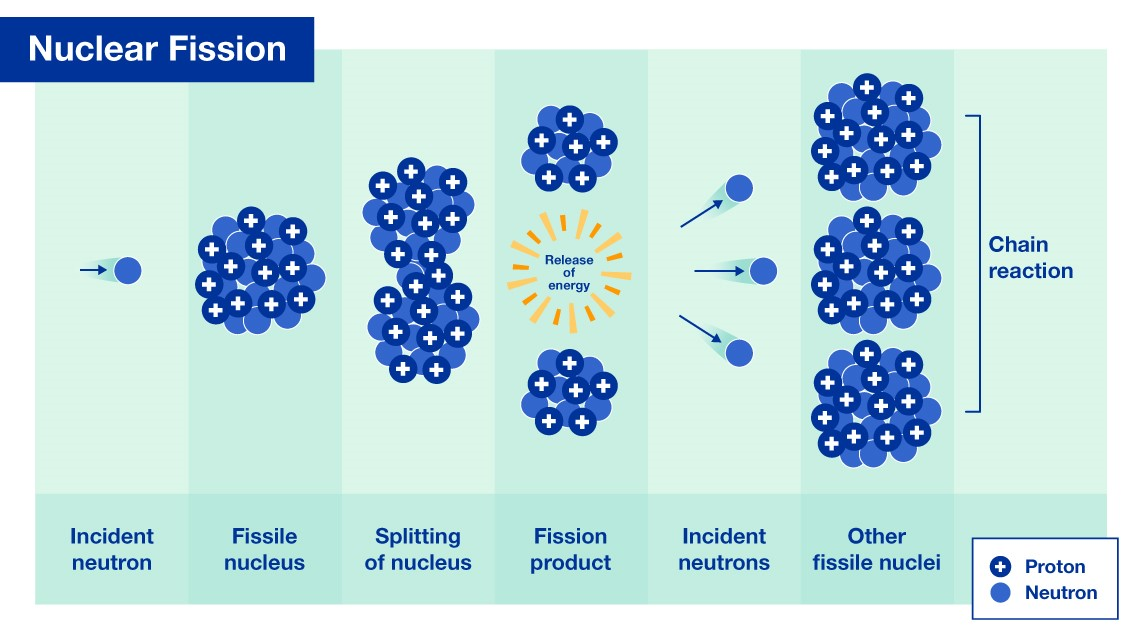
\includegraphics[width=\linewidth]{IAF.jpeg}
    \caption{An example of chain reaction\protect\footnotemark}
    \label{fig:enter-label}
\end{figure}

\footnotetext{https://www.iaea.org/newscenter/news/what-is-nuclear-energy-the-science-of-nuclear-power}

\item Fusion : in this mechanism two light atoms merge into a larger one and release additional energy.This is the the nuclear transformation that powers the sun.
\end{itemize}

\section{Nuclear energy power plants}
The first nuclear power plant was opened in 1954 in Obninsk in the Soviet Union.Since then worldwide we had three generations of power reactors and two additional generations are under deployment or research.In the following we will describe briefly each single generation.\footnote{https://www.amacad.org/sites/default/files/academy/pdfs/nuclearReactors.pdf}
\begin{figure}
    \centering
    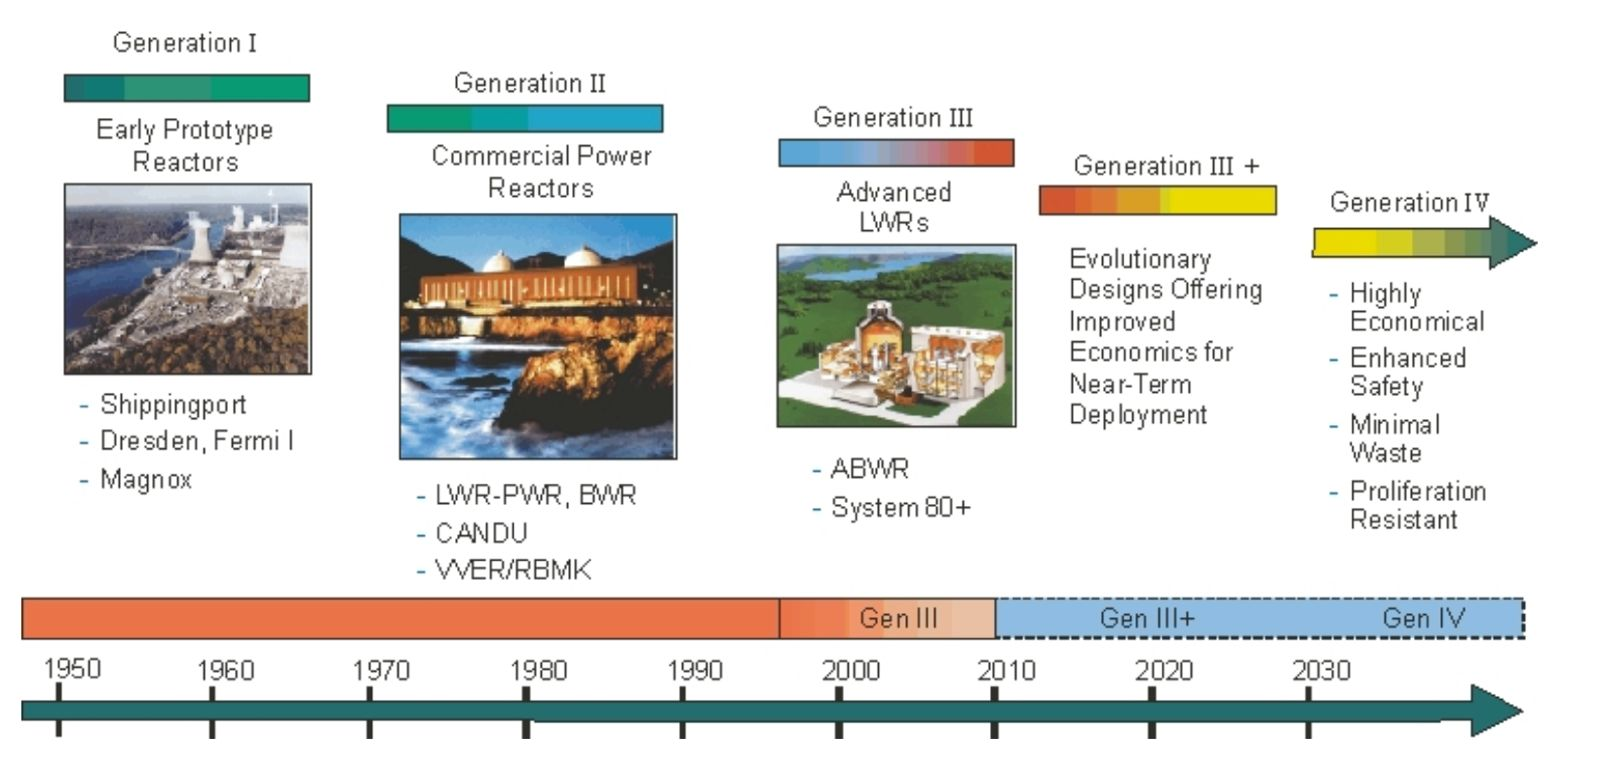
\includegraphics[width=1\linewidth]{WhatsApp Image 2024-02-11 at 22.11.21.jpeg}
    \caption{Timeline of nuclear power plants\protect\footnotemark}
    \label{fig:enter-label}
\end{figure}
\footnotetext{https://www.oecd-nea.org/science/rd/presentations/2-2-doc.pdf}

\subsection{Generation I}
It refers to early prototypes deployed in the U.S. and UK. As of 2024 reactors of this generation have been all decommissioned.

\subsection{Generation II}
They began operating in the late 1960s and are the most common ones. In the world at least 400 of these reactors were built.In the last 50 years these reactors have been improved in order to have additional safety systems and emergency power.

\subsection{Generation III}
There are basic improvements on Generation II and in particular the focus have been on modular constructions with the purpose to decrease costs.In addition the design was aimed to achieve at least an operational life of 60 years.

\subsection{Generation III+ and IV}
Nuclear power plants of generation III+ are in operation since 2010 and represent the state of the art in terms of safety and security.Generation IV are still in research or deployment phase and not operational yet. The main goal is to use alternative radioactive materials and different cooling systems.

\section{Advantages and disadvantages}
In the following there is a discussion about advantages and concerns of nuclear power plants.

\subsection{Advantages}
\begin{itemize}
    \item It's one of the cleanest energy sources in the world.
    Here is a proof:
    \begin{figure}
        \centering
        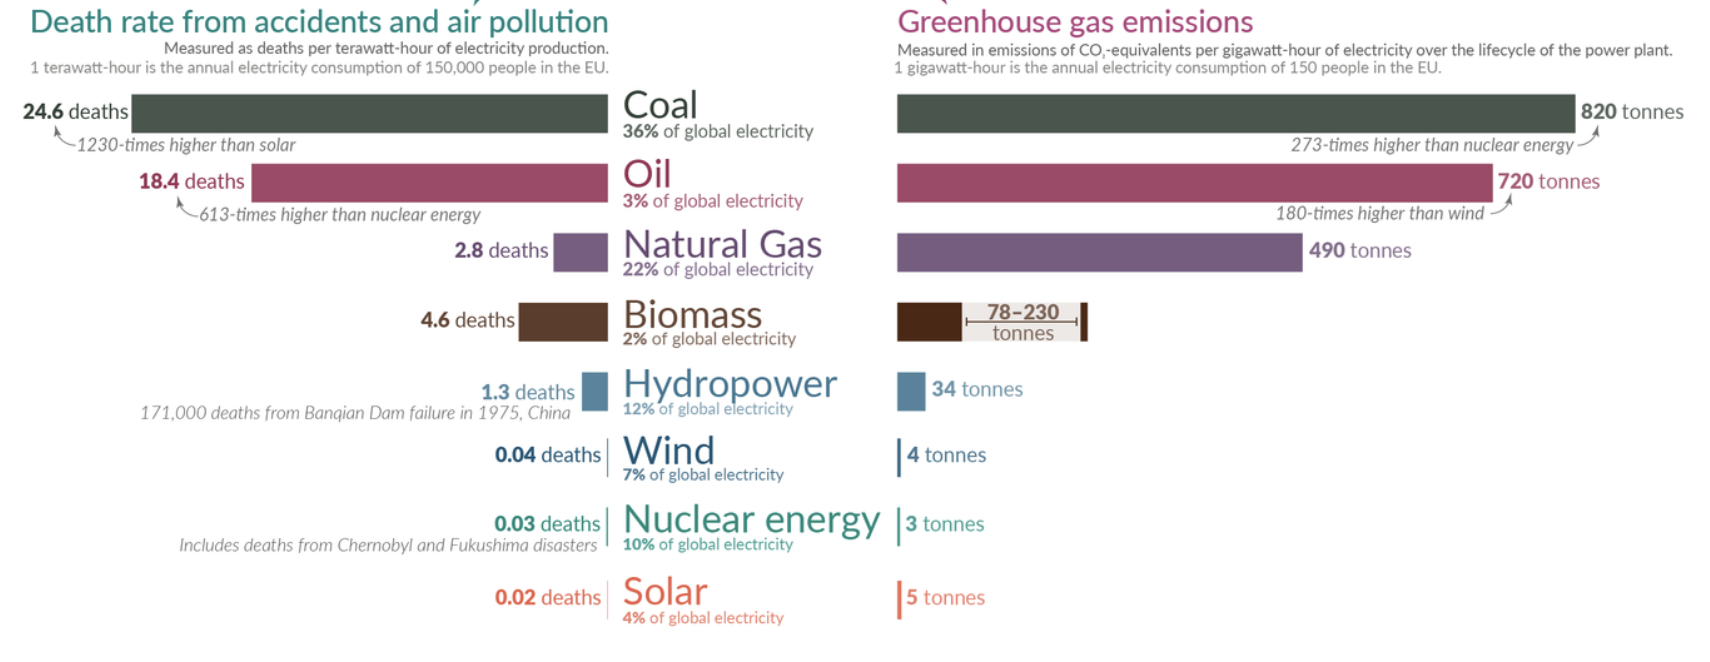
\includegraphics[width=1.39\linewidth]{AAAAASUKA.png}
        \caption{A chart showing all energy sources and how bad or good they are for the environment\protect\footnotemark.}
        \label{fig:enter-label}
    \end{figure}
    \footnotetext{https://ourworldindata.org/safest-sources-of-energy}

This chart shows that nuclear energy is cleaner than the most of the other energy sources.

\item Nuclear energy is safe.

Nuclear energy is safe. The construction of nuclear power plants is regulated with the highest international safety standards and monitored and certified by international authorities. When we talk about safety of nuclear power plants we must think of safety of flights as example. Although it is counter-intuitive, flights are much more safer than trains or cars and the same is for nuclear energy when compared to coal or gas.

\item Nuclear energy waist is not polluting air and therefore is not killing people.This is one of the main differences with respect to coal, gas, wood and oil.


\end{itemize}
\subsection{Disadvantages}
\begin{itemize}
    \item People are scared by nuclear energy (in the same way as they are scared by flights).This energy is very new, very far from what we are used to deal with every day,  and schools and governments are doing a very poor job in education regarding it.

    \item Uranium-235 is a finite resource. According to the Nuclear Energy Agency (NEA) our current supply of uranium might last for only 200 years and even nowadays it is not widely available. Although this is not an immediate concern it might become it in future as nuclear energy usage increases.
    \item Nuclear energy waist can be used for producing nuclear weapons and as a result of mismanagement can be a source of worldwide concerns.
    \item Nuclear technology is not widely available worldwide and requires very advanced specialised workers.
    
\end{itemize}
\section{Nuclear fusion}
In this paper we focused mostly on Nuclear fission however in the last 15 years very significant improvements have been done to nuclear fusion.This technology promises to solve all the cons mentioned above while generating even more energy. As this technology is not available nowadays we won't deep dive further.

\section{Conclusions}

The main result that we want to achieve with this paper is to not give a reccomendation or to influence the reader pro or against nuclear energy. We just attempted to provide some information in order to allow curious minds to be open and understand the world around us. The reader is encouraged to read all the references and make its own opinion.
\end{document}
